\documentclass{beamer}
\usetheme{Madrid}

\usepackage{tikz}
\usepackage{siunitx}

\title[Physics Problem Solving]{Physics Problem Solving}
\author{Dara Daneshvar \and Eason Shao \and Lev Shabalin}
\institute[]{Physics Problem Solving Society\\St Paul's School}
\date{29.04.2024}

\AtBeginSection[]
{
    \begin{frame}
        \frametitle{Table of Contents}
        \tableofcontents[currentsection]
    \end{frame}
}

\begin{document}

    \frame{\titlepage}
    
    \begin{frame}
        \frametitle{Table of Contents}
        \tableofcontents
    \end{frame}
    
    \section{Springs and Newton-metre}

    \begin{frame}{Question}
        This question aims to let us think what actually a Newton-metre measures.\pause

        \textit{(Surprisingly, it does not measure the newton metre, which is the joule.)}\pause

        \begin{block}{Question}
            Given that the following setup satisfies that $mg = 5 \si{N}$, find the reading of the Newton-metre in the following setups. \pause

            \begin{figure}
                \centering
                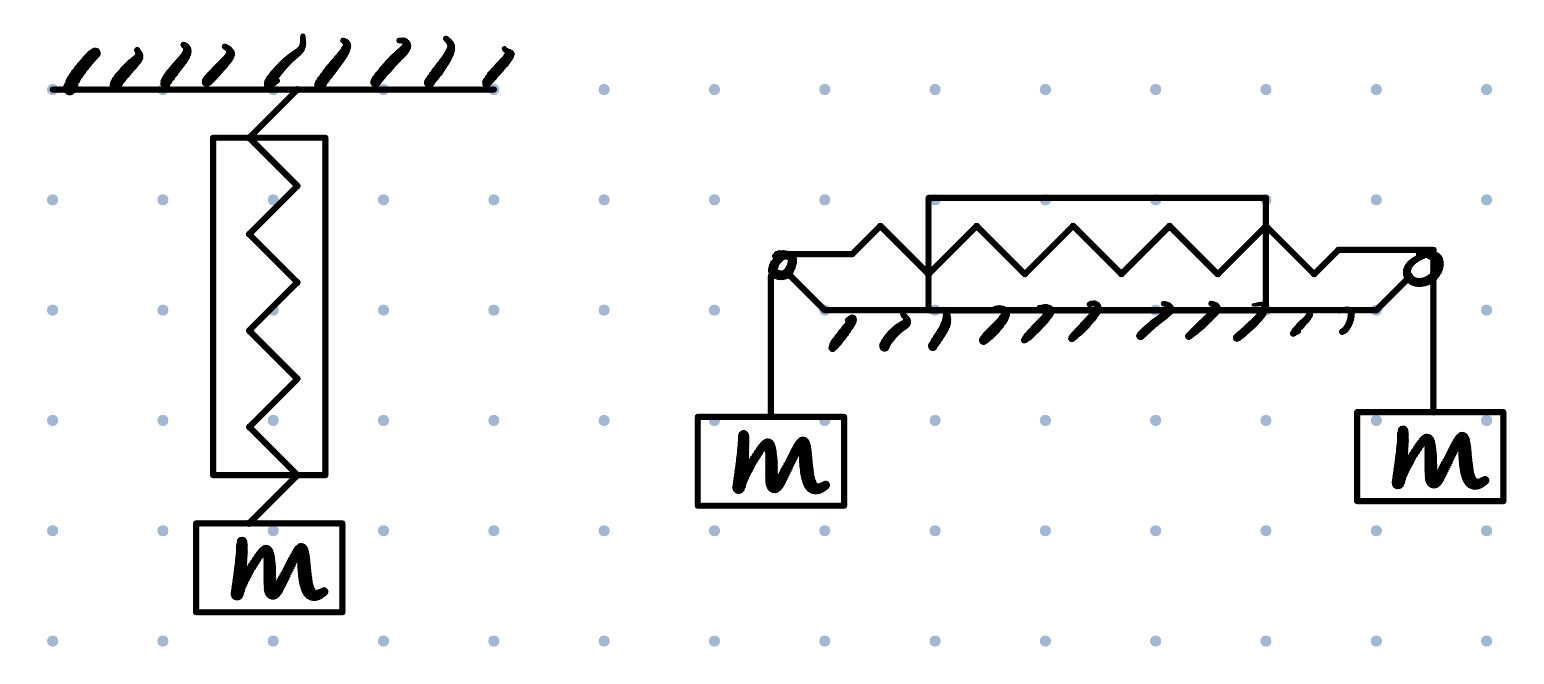
\includegraphics[width=0.5\textwidth]{diagram.jpg}
                \caption{Setup}
                \label{fig:SetupOfNewtonMetre}
            \end{figure}\pause

            \textit{You may assume that the Newton-metres are massless.}
        \end{block}
    \end{frame}

    \begin{frame}{Thoughts}
        \begin{exampleblock}{Thoughts}
            \begin{itemize}
                \item From our first glance, one may argue that the second setup has double the reading of the first setup, since it receives the same $5 \si{N}$ pull on both sides, therefore will receive a 'resultant' pull of $10 \si{N}$.\pause
    
                \item Also, by the fact that the Newton-metre measures the weight of an object in the first setup. we will see that it reads $5 \si{N}$ in the first setup.\pause
        
                \item However, after doing a force analysis on the Newton-metre in the first setup, unsurprisingly, we also found that it experiences $5 \si{N}$ pull on both sides.\pause
    
                \item Essentially the setup are equivalent.\pause
    
                \item \alert{What went wrong here?}
            \end{itemize}
        \end{exampleblock}
    \end{frame}

    \begin{frame}{Analysis}
        \begin{exampleblock}{Analysis}
            \begin{itemize}
                \item In an ideal world where all newton-metres are massless (which could not be the case in our real world), we will know that the resultant force that acts on the newton-metre is $0$.\pause

                \item Therefore, assuming it only has pull on both ends, they must be on the same straight line, act on opposite directions, and have \alert{equal magnitude}.\pause

                \item What the newton-metre actually reads is the pull on \alert{only one end}.\pause
                
                \item This is very reasonable, due to the first setup, and usually we hold the other end on a fixed end/with our hand, which we do not usually account for the pull twice.
            \end{itemize}
            
        \end{exampleblock}
    \end{frame}

    \section{Direction of Friction}

    \begin{frame}{Question}
        We know from GCSE Physics that friction is to oppose relative motion of two surfaces.

        In other words, static friction exists, if when the friction is removed the surfaces will slide relatively opposite to the direction of a friction.

        \begin{block}{Question}
            A person is climbing up along a climbing rope. Determine the direction of friction they experience.
        \end{block}
    \end{frame}

    \begin{frame}{Thoughts}
        \begin{exampleblock}{Thoughts}
            \begin{itemize}
                \item To our intuition, since I am climbing upwards on the rope, I must receive the friction downwards, which 'opposes' my motion. \pause

                \item However, if we draw a force diagram analysing this situation, we will see that there is \alert{no force pointing upwards}, and according to Newton, we can't climb up a rope. \pause

                \item \alert{What went wrong here?}
            \end{itemize}
        \end{exampleblock}
    \end{frame}

    \begin{frame}{Analysis}
        \begin{exampleblock}{Analysis}
            \begin{itemize}
                \item Let's do a thought experiment here. If the rope is smooth and does not have any friction, where will I go? \pause
                \item I hope it is obvious for everyone, that we will slide down the rope. \pause
                \item Therefore, to oppose this motion, the friction will have to act upwards.
            \end{itemize}
        \end{exampleblock}
    \end{frame}

    \begin{frame}{More Thoughts}
        \begin{exampleblock}{Thoughts}
            \begin{itemize}
                \item We are not done yet ... \pause
                \item It is \alert{not} very convincing that the friction can be the \alert{driving force} - shouldn't it just 'stop acting' when the relative motion stops and just 'maintain' the stop position - and act as a \alert{resisting force}? \pause
                \item \alert{What went wrong here?}
            \end{itemize}
        \end{exampleblock}
    \end{frame}

    \begin{frame}{More Analysis}
        \begin{exampleblock}{Analysis}
            \begin{itemize}
                \item We shall think carefully how a person climbs a rope. \pause
                \item Are the surfaces sliding at any time? Are the hands of the person sliding upwards against the rope at any time? \pause
                \item \alert{No.} Our hand, always tends to slide down from the rope. \pause
                \item In fact, we cannot model our body as a point mass in this question. We are moving our arms to climb. \pause
                \item When we climb up, one of our arms and some of our body remain stationary, while the other arm and most of our body accelerates upwards, thanks to the arm providing the force upwards. \pause
                \item The arms which remains stationary has to provide some extra upwards force to push the body upwards. To balance this, there is extra friction provided (extra in the sense of being equal to our weight).
            \end{itemize}
        \end{exampleblock}
    \end{frame}

    \section{Easter Question Pack}

    \begin{frame}{Question 4}
        \begin{block}{Question}
            A tank contains water to a depth of $1.0 \si{m}$. Water emerges from a small hole in the vertical side of the tank at $20 \si{cm}$ below the surface. Determine: 
            \begin{enumerate}
                \item the speed at which the water emerges from the hole 
                \item the distance from the base of the tank at which the water strikes the floor on which the tank is standing.
            \end{enumerate}
        \end{block}
    \end{frame}

    \begin{frame}{Solution}
        \begin{exampleblock}{Solution}
            Water is pushed out of the hole due to the weight of water above.\pause
            
            The velocity of water exiting the hole can be found using energy conservation, where gravitational potential energy is transferred to kinetic energy,
            \[mgh = \frac{1}{2}mv^2\]
            \[v^2 = 2gh.\] \pause
            Substituting values, with the height of water above the hole $h = 20\si{cm},$
            \[v = \sqrt{2 \times 9.81 \times 0.2} = 1.98 \si{m.s^{-1}}.\]
        \end{exampleblock}
    \end{frame}

    \begin{frame}{Solution}
        \begin{exampleblock}{Solution}
            Water exits the hole in the tank horizontally. It can then be modelled as a projectile as it falls to the ground. \pause
            
            Since the vertical velocity of the water is initially zero,
            \[s = \frac{1}{2} at^2 \;\Rightarrow\; t = \sqrt{\frac{2s}{g}}.\]\pause
            Substituting values,
            \[t = \sqrt{\frac{2 \times 0.8}{9.81}} = 0.404 \si{s}.\]\pause
            Now considering the horizontal motion of the water,
            \[d = 1.98 \times 0.404 = 0.80 \si{m} = 80 \si{cm}.\]
        \end{exampleblock}
    \end{frame}
    
\end{document}